\section{Введение}

\subsection{Цели работы}

\begin{itemize}
    \item исследовать эффект Холла в полупроводниках,
    \item определить концентрацию носителей заряда и их подвижность;
    \item определить знак носителей;
\end{itemize}

\subsection{Используемые приборы}

    Электромагнит с регулируемым источником питания, вольтметр, амперметр, миллиамперметр, милливеберметр, источник питания (1,5 В), образцы легированного германия;

\newpage

\section{Теоретическая часть}

\subsubsection{Эффект Холла}

Во внешнем магнитном поле \( B \) на заряды действует сила Лоренца:

\begin{equation}
\mathbf{F} = q\mathbf{E} + q\mathbf{u} \times \mathbf{B}
\end{equation}

Эта сила вызывает движение носителей, направление которого в общем случае не совпадает с полем \( \mathbf{E} \). В проводнике возникает поперечное электрического поле. Такое явление называется \textbf{эффектом Холла}.

\subsubsection{Тензор проводимости в магнитном поле}

Связь между электрическим полем \( \mathbf{E} \) и плотностью тока \( \mathbf{j} \) при эффекте Холла не может быть описана скалярным коэффициентом проводимости \( \sigma \). Закон Ома записывается в виде:

\begin{equation}
\mathbf{j} = \hat{\sigma} \mathbf{E}
\end{equation}

где \( \hat{\sigma} \) — это тензор проводимости, который в выбранной системе координат представляется в виде матрицы:

\begin{equation}
\hat{\sigma} =
\begin{pmatrix}
\sigma_{xx} & \sigma_{xy} & \sigma_{xz} \\
\sigma_{yx} & \sigma_{yy} & \sigma_{yz} \\
\sigma_{zx} & \sigma_{zy} & \sigma_{zz}
\end{pmatrix}
\end{equation}

Для случая одного типа носителей (например, электронов) и плоской геометрии:

\begin{figure}[H]
    \centering
    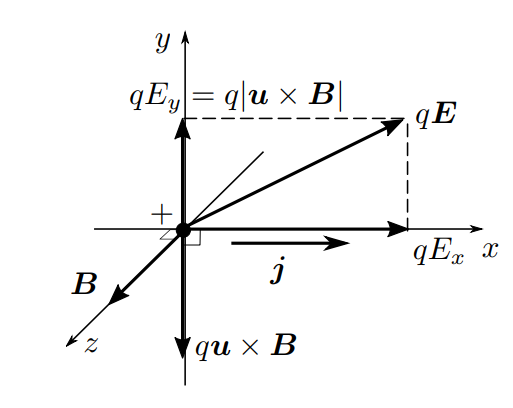
\includegraphics[width=0.5\textwidth]{pictures/r2.png}
\end{figure}

\begin{equation}
E_y = u_x B_z = \frac{j_x B_z}{nq}
\end{equation}

Плотность тока вдоль оси \( x \) описывается формулой:

\begin{equation}
j_x = qnu_x = qn\mu E_x = \sigma_0 E_x
\end{equation}

где \( \sigma_0 = nq\mu \) — удельная проводимость среды в отсутствие магнитного поля \( B \). 

Обобщённый закон Ома при наличии внешнего магнитного поля:

\begin{equation}
\mathbf{E} = \frac{\mathbf{j}}{\sigma_0} - \frac{1}{nq} (\mathbf{j} \times \mathbf{B})
\end{equation}

В компонентной форме для случая одного типа носителей (вдоль оси z):

\begin{equation}
E_x = \frac{j_x}{\sigma_0} - \frac{j_y B}{nq}, \quad E_y = \frac{j_y}{\sigma_0} + \frac{j_x B}{nq}, \quad E_z = \frac{j_z}{\sigma_0}
\end{equation}

Тензор удельного сопротивления \( \hat{\rho} \), обратный тензору проводимости, принимает вид:

\begin{equation}
\hat{\rho} =
\frac{1}{\sigma_0}
\begin{pmatrix}
1 & -\mu B & 0 \\
\mu B & 1 & 0 \\
0 & 0 & 1
\end{pmatrix}
\end{equation}

Тензор проводимости:

\begin{equation}
\hat{\sigma} = \frac{\sigma_0}{1 + (\mu B)^2}
\begin{pmatrix}
1 & \mu B & 0 \\
-\mu B & 1 & 0 \\
0 & 0 & 1
\end{pmatrix}
\end{equation}

\subsubsection{Мостик Холла}

\begin{figure}[H]
    \centering
    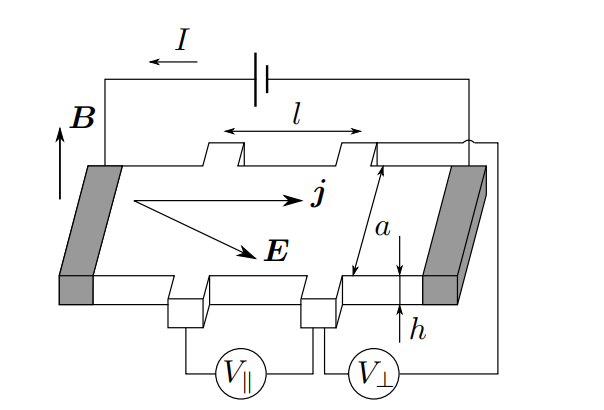
\includegraphics[width=0.6\textwidth]{pictures/r3.png}
    \caption{Мостик Холла}
\end{figure}

В схеме мостика Холла ток течёт вдоль оси \( x \) по плоской пластинке, помещённой в магнитное поле, направленное перпендикулярно пластинке. Возникает поперечное электрическое поле, создающее напряжение Холла:

\begin{equation}
U_\perp = E_ya = \frac{j_x B a}{n q} = \frac{B}{nqh} I = R_H \cdot \frac{B}{h} \cdot I
\end{equation}

где \( R_H = \frac{1}{nq} \) — постоянная Холла.

Продольное напряжение:

\begin{equation}
U_\parallel = E_x l = \frac{j_x l}{\sigma_0} = I R_0
\end{equation}

где \( R_0 = \frac{l}{\sigma_0 a h} \) — омическое сопротивление образца.

\subsection{Экспериментальная установка}

Электрическая схема установки для измерения ЭДС Холла представлена на рис. \ref{r1}. В зазоре электромагнита (рис. \ref{r1}а) создаётся постоянное магнитное поле, величина которого регулируется источником питания, а ток измеряется амперметром \(A_1\). Направление тока в обмотках можно изменить, переключив разъём \(K_1\).

Градуировка электромагнита проводится с помощью милливеберметра или миллитесламетра.

Прямоугольный образец из легированного германия (рис. \ref{r1}б) подключается к источнику питания (\(\approx 1.5 \, \text{В}\)). При замыкании ключа \(K_2\) по образцу течёт ток, величина которого регулируется реостатом \(R_2\) и измеряется миллиамперметром \(A_2\). Разность потенциалов \(U_{34}\) между контактами 3 и 4 измеряется вольтметром \(V\).

\begin{figure}[H]
    \centering
    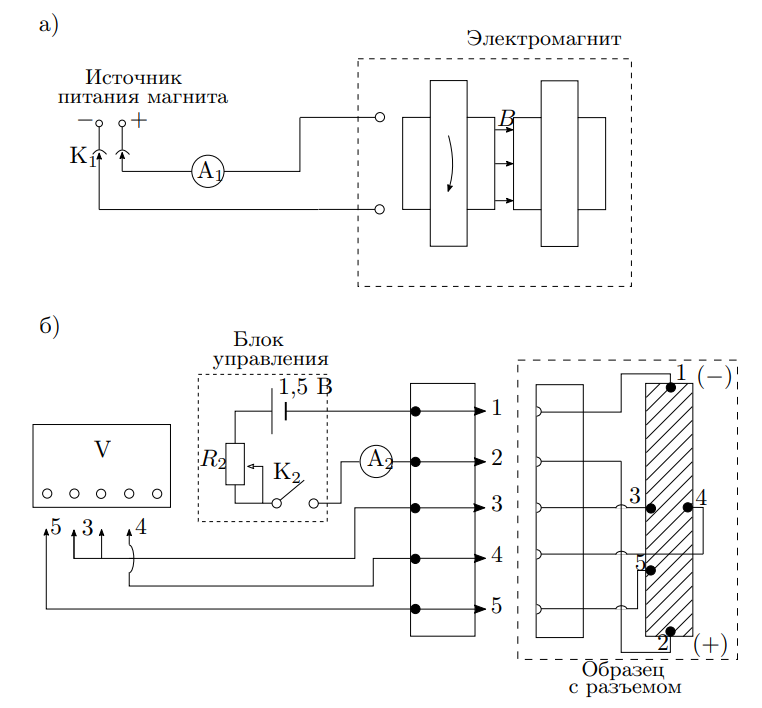
\includegraphics[width=0.7\textwidth]{pictures/r1.png}
    \caption{Схема установки для исследования эффекта Холла: (а) электромагнит; (б) держатель с образцом.}
    \label{r1}
\end{figure}

Контакты 3 и 4 могут не лежать на одной эквипотенциали из-за неточности подпайки. Чтобы исключить влияние омического падения напряжения, меняется направление магнитного поля. ЭДС Холла \(U_\perp\) определяется как:

\begin{equation}
    U_\perp = U_{34} - U_0
\end{equation}

Измерив ток \( I \) и напряжение \( U_{35} \) между контактами 3 и 5 в отсутствие магнитного поля, проводимость материала рассчитывается по формуле:

\begin{equation}
    \rho_0 = \frac{U_{35} a h}{I l}
\end{equation}

где \( l \) — расстояние между контактами 3 и 5, \( a \) — ширина образца, \( h \) — его толщина.
